\documentclass[aspectratio=169,11pt]{beamer}

\usetheme{default}
\setbeamertemplate{navigation symbols}{}
\setbeamertemplate{footline}[frame number]

\usepackage[T1]{fontenc}
\usepackage{lmodern}
\usepackage{hyperref}
\usepackage{xcolor}
\usepackage{listings}
\usepackage{tikz}

% --- Listings style (uncluttered, code-forward) ---
\definecolor{CodeBg}{RGB}{248,248,248}
\definecolor{CodeFrame}{RGB}{220,220,220}
\definecolor{CodeKeyword}{RGB}{0,90,180}
\definecolor{CodeComment}{RGB}{110,110,110}
\definecolor{CodeString}{RGB}{140,60,0}

\lstset{
  language=Python,
  basicstyle=\ttfamily\small,
  keywordstyle=\color{CodeKeyword}\bfseries,
  commentstyle=\color{CodeComment},
  stringstyle=\color{CodeString},
  showstringspaces=false,
  backgroundcolor=\color{CodeBg},
  frame=single,
  rulecolor=\color{CodeFrame},
  frameround=tttt,
  breaklines=true,
  tabsize=2,
  columns=fullflexible
}

\title{Apache Arrow in Python}
\subtitle{A practical introduction to \texttt{pyarrow}}
\author{}
\date{}

\begin{document}

% --- Title ---
\begin{frame}
  \titlepage
\end{frame}

% --- Motivation ---
\begin{frame}{Why Arrow?}
\vspace{2mm}
\begin{itemize}
  \item A \textbf{columnar in-memory format} for analytics
  \item Designed for \textbf{zero-copy sharing} across systems/languages
  \item A toolbox: \textbf{I/O (Parquet/IPC)}, \textbf{compute kernels}, \textbf{dataset scanning}
\end{itemize}
\end{frame}

% --- Mental model ---
\begin{frame}{Mental model (keep this picture in mind)}
\begin{itemize}
  \item \textbf{Typed columns} (\texttt{int64}, \texttt{timestamp}, \texttt{string}, \ldots)
  \item Data stored in \textbf{contiguous buffers} (+ optional \textbf{validity bitmap} for nulls)
  \item Tables are \textbf{collections of equal-length columns}
\end{itemize}
\end{frame}

% --- Install / import ---
\begin{frame}[fragile]{Install + import}
\begin{lstlisting}
# Recommended:
pip install "pyarrow>=14"

import pyarrow as pa
import pyarrow.compute as pc
\end{lstlisting}
\end{frame}

% --- Core objects ---
\begin{frame}{Core objects you’ll see everywhere}
\begin{itemize}
  \item \textbf{\texttt{pa.Array}}: a typed column (nullable)
  \item \textbf{\texttt{pa.ChunkedArray}}: one logical column split into chunks
  \item \textbf{\texttt{pa.RecordBatch}}: columns + schema (batch of rows)
  \item \textbf{\texttt{pa.Table}}: columns + schema (many batches/columns)
\end{itemize}
\end{frame}

% --- Arrays / types ---
\begin{frame}[fragile]{Arrays + explicit types}
\begin{lstlisting}
import pyarrow as pa

a = pa.array([1, 2, None, 4], type=pa.int64())
b = pa.array(["nyc", "sf", None, "la"], type=pa.string())

a.type, b.type
# (DataType(int64), DataType(string))
\end{lstlisting}
\end{frame}

% --- Table / schema ---
\begin{frame}[fragile]{Tables + schema}
\begin{lstlisting}
import pyarrow as pa

t = pa.table(
    {
        "pickup_zone": ["Midtown", "Midtown", "SoHo"],
        "fare": [12.5, 18.0, 9.25],
        "hour": [8, 9, 8],
    },
    schema=pa.schema([
        ("pickup_zone", pa.string()),
        ("fare", pa.float64()),
        ("hour", pa.int8()),
    ])
)

t.schema
\end{lstlisting}
\end{frame}

% --- Pandas interoperability ---
\begin{frame}[fragile]{Pandas interop (focus: controlling copies)}
\begin{lstlisting}
import pandas as pd
import pyarrow as pa

df = pd.DataFrame({"x": [1, 2, None], "y": ["a", "b", None]})

# Pandas -> Arrow
t = pa.Table.from_pandas(df, preserve_index=False)

# Arrow -> Pandas (copy behavior depends on dtype)
df2 = t.to_pandas()
\end{lstlisting}
\end{frame}

% --- Parquet I/O ---
\begin{frame}[fragile]{Parquet I/O (fast + columnar)}
\begin{lstlisting}
import pyarrow as pa
import pyarrow.parquet as pq

t = pa.table({"a": [1, 2, 3], "b": ["x", "y", "z"]})

pq.write_table(t, "example.parquet")

t2 = pq.read_table("example.parquet", columns=["a"])
\end{lstlisting}
\end{frame}

% --- Why Parquet/Arrow I/O is fast ---
\begin{frame}{Why Arrow often makes I/O feel fast}
\begin{itemize}
  \item \textbf{Columnar read}: only load requested columns (\textit{projection})
  \item \textbf{Skip work}: statistics + row groups enable \textit{predicate pushdown} (read fewer bytes)
  \item \textbf{Efficient encoding}: dictionary / RLE / bit-packing reduce bytes-to-read
  \item \textbf{Vectorized decode}: tight loops convert bytes $\rightarrow$ typed arrays efficiently
  \item \textbf{Parallelism}: row groups can be read/decoded in parallel
\end{itemize}
\end{frame}

% --- Dataset scanning ---
\begin{frame}[fragile]{Datasets: scan with projection + filter}
\begin{lstlisting}
import pyarrow.dataset as ds

dataset = ds.dataset("example.parquet", format="parquet")

# Read only what you need:
scanner = dataset.scanner(
    columns=["a"],
    filter=(ds.field("a") >= 2)
)

tbl = scanner.to_table()
\end{lstlisting}
\end{frame}

% --- Compute kernels ---
\begin{frame}[fragile]{Compute kernels (vectorized, typed)}
\begin{lstlisting}
import pyarrow as pa
import pyarrow.compute as pc

arr = pa.array([1, 2, None, 4])

pc.sum(arr)                 # scalar result
pc.fill_null(arr, 0)        # array result
pc.equal(arr, 2)            # boolean mask
\end{lstlisting}
\end{frame}

% --- Strings & dictionary encoding ---
\begin{frame}[fragile]{Categoricals: dictionary encoding}
\begin{lstlisting}
import pyarrow as pa

cities = pa.array(["NYC", "SF", "NYC", "LA", "NYC"])
cat = cities.dictionary_encode()

cat.type
# dictionary<values=string, indices=int32, ordered=0>
\end{lstlisting}
\end{frame}

% --- IPC / Feather ---
\begin{frame}[fragile]{IPC / Feather: share Arrow data on disk}
\begin{lstlisting}
import pyarrow as pa
import pyarrow.feather as feather

t = pa.table({"x": [1, 2, 3], "y": ["a", "b", "c"]})

feather.write_feather(t, "example.feather")
t2 = feather.read_table("example.feather")
\end{lstlisting}
\end{frame}

% --- Why IPC / Feather is fast ---
\begin{frame}{Why Arrow IPC / Feather is fast (local interchange)}
\begin{itemize}
  \item \textbf{No text parsing}: it’s already typed, binary columnar data
  \item \textbf{Zero-/low-copy}: contiguous buffers can often be memory-mapped
  \item \textbf{Cheap slicing}: many operations are views over the same buffers
  \item \textbf{Interop}: avoids repeated conversions between tool-specific formats
\end{itemize}
\end{frame}

% --- Practical tips ---
\begin{frame}{Practical tips (avoid surprises)}
\begin{itemize}
  \item \textbf{Chunking}: some operations return \texttt{ChunkedArray} — use \texttt{combine\_chunks()} if needed
  \item \textbf{Nulls are first-class}: types are nullable by default
  \item \textbf{Be explicit about types} for timestamps/timezones/large strings
\end{itemize}
\end{frame}

% --- When to use Arrow ---
\begin{frame}{When Arrow shines}
\begin{itemize}
  \item Scanning big columnar data (Parquet) with projection + filtering
  \item Interop: moving data between tools (Pandas/Polars/DuckDB/Spark)
  \item Standardizing schemas + types across pipelines
\end{itemize}
\end{frame}


% --- Arrow-Dask Integration ---
\begin{frame}{Arrow and Dask Integration}
\small
\textbf{Apache Arrow:}
\begin{itemize}
    \item Columnar in-memory format for analytics
    \item Designed for zero-copy data sharing
    \item Cross-language interoperability
    \item Efficient serialization format
\end{itemize}

\vspace{0.1cm}
\textbf{Why Arrow Matters for Dask:}
\begin{itemize}
    \item Efficient data transfer between workers
    \item Reduced memory usage (especially strings)
    \item Fast Parquet I/O operations
    \item Better performance for large datasets
\end{itemize}
\end{frame}

\begin{frame}{Zero-Copy Data Transfer}
\small
\textbf{Traditional Approach (with copies):}
\begin{itemize}
    \item Worker 1: Serialize data $\rightarrow$ bytes
    \item Network: Transfer bytes
    \item Worker 2: Deserialize bytes $\rightarrow$ data
    \item \textbf{Problem:} Multiple copies, slow
\end{itemize}

\vspace{0.1cm}
\textbf{Arrow Approach (zero-copy):}
\begin{itemize}
    \item Data in Arrow format (columnar)
    \item Transfer memory buffers directly
    \item No serialization/deserialization overhead
    \item \textbf{Benefit:} Faster, less memory
\end{itemize}

\vspace{0.05cm}
\begin{center}
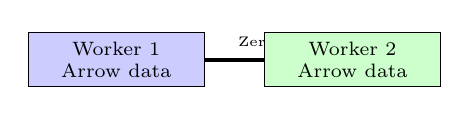
\begin{tikzpicture}[scale=0.5, every node/.style={font=\scriptsize}]
    % Worker 1
    \node[draw, rectangle, fill=blue!20, text width=2cm, align=center] (w1) at (-3,0) {Worker 1\\Arrow data};
    % Arrow
    \draw[->, very thick] (w1) -- node[above, font=\tiny] {Zero-copy} (3,0);
    % Worker 2
    \node[draw, rectangle, fill=green!20, text width=2cm, align=center] (w2) at (3,0) {Worker 2\\Arrow data};
\end{tikzpicture}
\end{center}
\end{frame}

\begin{frame}[fragile]{Arrow-Backed Dtypes}
\small
\textbf{Memory Efficiency:}
\begin{itemize}
    \item Arrow-backed strings: Up to 70\% less memory
    \item Especially important for Dask clusters
    \item Reduces memory pressure significantly
\end{itemize}

\begin{lstlisting}
import pandas as pd
import dask.dataframe as dd

# Create DataFrame with Arrow-backed strings
df = pd.DataFrame({
    'name': pd.array(['Alice', 'Bob'], dtype='string[pyarrow]'),
    'value': [1, 2]
})

# Dask automatically uses Arrow format
ddf = dd.from_pandas(df, npartitions=2)
\end{lstlisting}

\textbf{Benefits:} Lower memory usage, faster operations, better performance
\end{frame}

\begin{frame}[fragile]{Parquet I/O with Arrow Engine}
\small
\textbf{Dask uses Arrow for Parquet:}
\begin{itemize}
    \item Default engine: \texttt{pyarrow} (Arrow-based)
    \item Alternative: \texttt{fastparquet} (legacy)
    \item Arrow provides better performance
\end{itemize}

\begin{lstlisting}
import dask.dataframe as dd

# Read Parquet with Arrow engine (default)
df = dd.read_parquet('data/*.parquet', engine='pyarrow')
\end{lstlisting}
\end{frame}

\begin{frame}{Parquet I/O with Arrow Engine - Features}
\small
\textbf{Arrow Enables:}
\begin{itemize}
    \item Column projection (read only needed columns)
    \item Predicate pushdown (filter at read time)
    \item Parallel I/O across partitions
    \item Efficient compression/decompression
\end{itemize}

\vspace{0.1cm}
\textbf{Key Features:}
\begin{itemize}
    \item Fast columnar reads
    \item Efficient filtering
    \item Parallel processing
\end{itemize}
\end{frame}

\begin{frame}{Arrow for Inter-Worker Communication}
\small
\textbf{Distributed Dask with Arrow:}
\begin{itemize}
    \item Workers communicate using Arrow format
    \item Data stays in Arrow format during transfer
    \item No conversion overhead
    \item Efficient for columnar data
\end{itemize}

\begin{center}
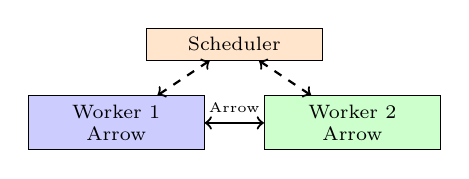
\begin{tikzpicture}[scale=0.5, every node/.style={font=\scriptsize}]
    % Scheduler
    \node[draw, rectangle, fill=orange!20, text width=2cm, align=center] (sched) at (0,2) {Scheduler};
    
    % Worker 1
    \node[draw, rectangle, fill=blue!20, text width=2cm, align=center] (w1) at (-3,0) {Worker 1\\Arrow};
    
    % Worker 2
    \node[draw, rectangle, fill=green!20, text width=2cm, align=center] (w2) at (3,0) {Worker 2\\Arrow};
    
    % Connections
    \draw[<->, thick, dashed] (sched) -- (w1);
    \draw[<->, thick, dashed] (sched) -- (w2);
    \draw[<->, thick] (w1) -- node[above, font=\tiny] {Arrow} (w2);
\end{tikzpicture}
\end{center}

\textbf{Benefits:} Faster transfer, lower memory, better scalability
\end{frame}

\begin{frame}{Arrow-Dask Integration: Summary}
\small
\textbf{Key Advantages:}
\begin{itemize}
    \item \textbf{Zero-copy transfers:} Efficient worker communication
    \item \textbf{Memory efficiency:} Arrow-backed strings use less memory
    \item \textbf{Fast I/O:} Optimized Parquet reading/writing
    \item \textbf{Columnar format:} Aligns with Dask's partition model
\end{itemize}

\textbf{When Arrow Shines:}
\begin{itemize}
    \item Large string columns (70\% memory savings)
    \item Distributed computations (zero-copy transfers)
    \item Parquet I/O operations (fast columnar reads)
    \item Cross-language workflows (standard format)
\end{itemize}

\textbf{Best Practice:} Use Arrow-backed dtypes, prefer \texttt{pyarrow} engine, leverage Arrow in distributed setups
\end{frame}


% --- Resources ---
\begin{frame}{Resources}
\begin{itemize}
  \item Docs: \texttt{https://arrow.apache.org/docs/python/}
  \item \texttt{pyarrow.dataset}: scalable scans
  \item \texttt{pyarrow.compute}: vectorized kernels
\end{itemize}
\end{frame}

\end{document}


